\section{A Synthesized and Refined View of Assurances} \label{sec:synthesis}
    %%%\edit{BRING IN SOME MATERIAL FROM LIPTON, GUNNING, WELLER, AND DOSHI-VELEZ}
    From the review of Quadrants I. through IV. of the formal/informal, explicit/implicit plane, we are able to find some insights with respect to assurances and can discuss them in a more comprehensive way. Using insights from the survey a refined version of Figure~\ref{fig:SimpleTrust_one_way} can be constructed. Figure~\ref{fig:refined_assurances} incorporates all details from Section~\ref{sec:background} as well as adding some insights from the survey that give direction about the design of assurances in human-AIA trust relationships. 
   
   Below we synthesize and discuss the design of explicit assurances in this more detailed framework -- some of these insights might also apply to implicit assurances, but will not be considered here along this line. %but implicit assurances will not be directly discussed in this paper.

    \begin{figure}[htbp]
        \centering
        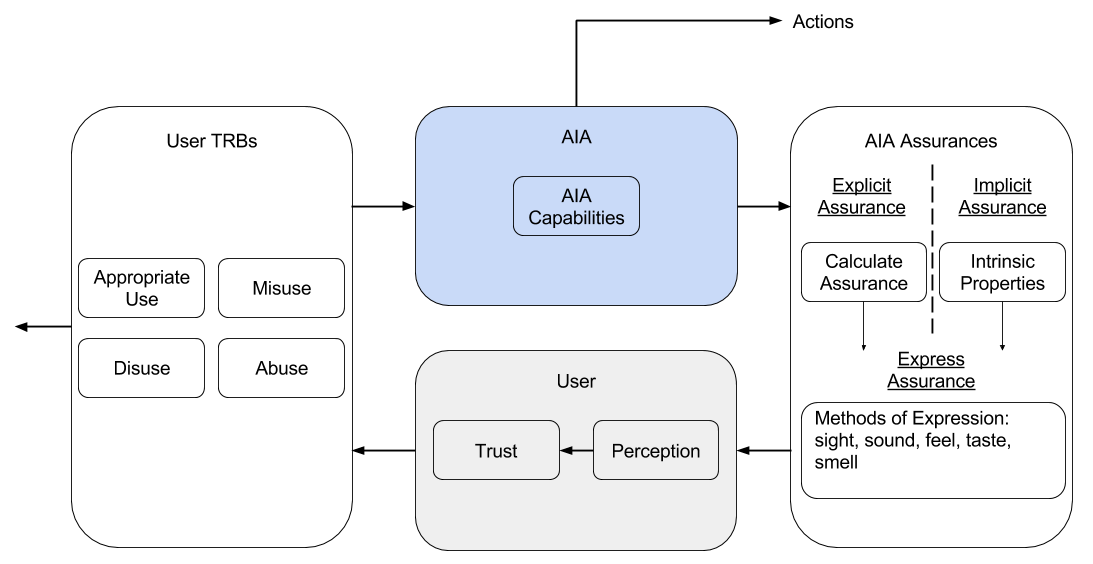
\includegraphics[width=0.65\textwidth]{Figures/RefinedTrust_one_way}
        \caption{Detailed extension of Figure~\ref{fig:SimpleTrust_one_way}. The AIA, User , and User TRBs blocks are defined as in Section~\ref{sec:background} (with the exception of the `Perception' blocks added to the AIA and User boxes). The AIA Assurances box has been filled using insights from the survey. The dark grey boxes will not be discussed; we focus on elements that a designer can address given an AIA with a fixed set of capabilities.}
        \label{fig:refined_assurances}
    \end{figure}

\subsection{Calculating, Designing, and Planning Explicit Assurances}
    Recall that an assurance is defined as \emph{any} behavior or property of an AIA that affects a user's trust; an explicit assurance is any assurance that was consciously implemented/applied by the designer with the express intention of influencing a user's TRBs/trust (whether or not the means for doing so conforms to a formal trust concept). As such, it is possible to design assuring properties into the system a priori. It is likewise possible to design assuring behaviors into an AIA. From the literature, several key high-level issues emerge pertaining to assurance implementation: (1) uncertainty quantification; (2) complexity reduction; (3) assurance by design; and (4) planning strategies for assurances. 

%     \begin{itemize}
%         \item Quantifying Uncertainty
%         \item Reducing Complexity
%         \item Assurance by Design
%         \item Planning Strategies of Assurance
%     \end{itemize}

    \paragraph{Quantifying Uncertainty} %%nra: awkward sentence: Being able to quantify the different kinds of uncertainty in the AIA is necessary before attempting to express that uncertainty to a human user. 
An AIA must have some way to assess and quantify uncertainty before attempting to express those uncertainties to a human user. 
There are several different kinds of uncertainty that might be considered, e.g. uncertainty in sensing, uncertainty in planning, and uncertainty in locomotion. 
A model or method needs to be incorporated in the AIA that will represent the different kinds of uncertainty to the human user in some way. 
A human user could use such information to inform their trust in the `situational normality', `competence', and/or `predictability' of the AIA. 
One might imagine that, in the UGV road-network problem, the UGV expressing high uncertainty in its plan would influence the competence component of the user's trust. Conversely, if an uncertainty measure is not available, the user might take this as an implicit assurance that the AIA is perfectly confident, or (based on the user's experience)  might conclude that since all AIA plans have been flawed in the past, the plan of this AIA must be flawed as well. 

The surveyed literature  featured several different uncertainty quantification approaches. In some cases uncertainty is already represented intrinsically by the algorithms and/or models being used in the AIA. Some use the built-in statistical representations of state transitions and sensor observations, e.g. for POMDPs, as the basis of quantifying uncertainty. This approach has straightforward analogs in other systems that use algorithms and/or models that inherently consider uncertainty. Models and methods that intrinsically represent uncertainty are frequently available. However, even when that it is the case, there are types of uncertainties that may still not be considered. For example, there are additional aspects of uncertainty beyond those intrinsically captured by some optimal planning approaches \cite{Aitken2016-fb,Kuter2012-bv}. 
Using the UGV road network problem as an example, what is the total probability distribution over all possible total cumulative reward outcomes (i.e. beyond just the expected value maximized by the optimal policy)? 
Or, given a certain road network, how closely can a Monte Carlo-based POMDP solver for the UGV approximate the true optimal policy? 
These describe `uncertainties in application', which arise in applying certain algorithms and models in different contexts.

Independent of the algorithms or representations used by an AIA, uncertainty quantification for assurance design also often focuses on assessing the probability of error for decision making as it pertains to any of the AIA capabilities from Fig. \ref{fig:AIcapabilities}. 
%(regression methods have analogous approaches). 
For instance, the problem of assessing the probability of error for classification and regression tasks for learning and perception are well-studied. 
In addition to standard training/validation data-based assessment techniques, some have approached this problem by learning models of errors for underlying learning models, e.g. by training a GP error `meta-model' for classifier errors  from empirical training data and using the meta-model to quantify uncertainty in different test scenarios \cite{Gurau2016-hs}. 
In contrast, we might quantify the uncertainty of a classifier based solely on the input data itself \cite{Zhang2014-he}. Of course, these methods share common drawbacks of being solely supervised learning approaches. However even in domains such as reinforcement learning, methods for avoiding highly uncertain (un-safe) rewards must use some form of external expert knowledge (see \cite{Garcia2015-rs, Lipton2016-dq}). Hence, the problem of defining a sensible `ground truth' against which uncertainties can be `correctly' assessed remains a fundamental challenge. %for developing AIA assurances.  
%
%\edit{...merge this paragraph with end of previous somehow...}
%    Uncertainty can be easier to assess if some kind of oracle, or reference is available for comparison. 

Some works have proposed quantifying the similarity between empirical experience and available reference data from a truth model as a measure of uncertainty \cite{Kaipa2015-hy}. Of course, this approach loses its appeal when a `truth model' isn't available. This shouldn't detract from the intent of finding some kind of reference (truth or otherwise) in which the reasoning, sensing, and other processes of an AIA can be compared to evaluate uncertainty. The evaluation of statistical models involves a very similar concept: given a statistical model as a reference does current empirical experience support or detract from the hypothesis that the model is still valid \cite{Laskey1995-jp,Ghosh2016-dl}? These approaches can quantify the degree to which the statistical models are still true, and this measurement can be used as an indication of uncertainty. However, these techniques can only provide binary indications that a model is statistically valid/invalid, without providing specific human-understandable causes or justifications as to why. Human expertise and designer judgment is thus required to carefully interpret such assurances, although a universal set of `best practices' for reporting such assurances and coping with cognitive biases in probabilistic/statistical data interpretation (framing effects, etc.) have yet to be established. 
%
%%This paragraph repeats the first one, so merging in the last part with that and commenting out the rest:
%%Generally, uncertainty quantification allows AIAs to express assurances related to the `situational normality', `competence', and `predictability' of the system in a given situation. One might imagine that, in the UGV road-network problem, the UGV expressing high uncertainty in its plan would influence the competence component of the user's trust. Conversely, if an uncertainty measure is not available, the user might take this as an implicit assurance that the AIA is perfectly confident, or (based on the user's experience)  might conclude that since all AIA plans have been flawed in the past, the plan of this AIA must be flawed as well.
%%
    \paragraph{Reducing Complexity} Many researchers have attempted to remove complexity from the models and logic of the AIA to make the methods more interpretable (or comprehensible, or explainable, \ldots) to human users. 
As with uncertainty quantification, interpretability can also inform a user's trust regarding the AIA's `situational normality', `competence', and `predictability'. Of course, this presupposes that many of the methods used by AIAs are `complex' by some measure; we claim that the fact that highly trained and educated experts are required to understand and develop these methods %(and even then it may not be totally possible) 
proves this supposition. Complexity only exists in the presence of some reference frame, i.e. the designer's or the user's in this case. 
From the perspective of an assurance designer, the key challenges to making/discovering/learning assurances with scalable interpretability lie in defining and satisfying criteria for required depth of understanding on the part of the user, the level of user expertise, and the time required by the user to gain understanding. 

Generally, the `complexity' of an algorithm or more general process used by an AIA is said to increase with the number of variables, steps of reasoning, the size of data, etc. in the formal sense that is understood by computer scientists. 
In practice, \textit{reduction} of complexity has been addressed by approaches as simple as finding summary statistics, e.g. calculating averages \cite{Muir1994-ow,Muir1996-gt}, that help explain why/how an algorithm or AIA arrives at a particular result. 
This can also be accomplished by computing heuristic measures which reduce many complex algorithmic components into more manageable pieces\cite{Aitken2016-fb}. Creating variable fidelity models is another way by which complexity can be reduced (and increased when necessary). One might also elect to create and use models to support AIA reasoning, decision, making, etc. capabilities which are inherently more interpretable to humans \cite{Caruana2015-za}. This could include constraining the feature space to be more simple, reducing dimensionality, learning more understandable features, and using physical theories to ground learned models (e.g. for interpretable science).  %%\edit{...merge? feels a bit out of place...}
    
It is possible for `inherently interpretable models and algorithms' to compete with other non-interpretable models in terms of performance. 
However, this may not be the most viable long-term approach for tackling the problem of complexity reduction in assurance design, especially due to the amount of work required to design interpretable counterparts to the latest state of the art algorithms for implementing AIA capabilities. 
On the other hand, approaches that seek `post hoc' explanations of complex models and algorithms offer more promise. 
This is partly because the idea of `interpretability' is not universally well-defined, and thus does not offer a single tangible goal. Rather, there exists a continuum of interpretability based on the complexity of the problem, the time required for a user to interpret (e.g. a few seconds vs. a few months of study, depending on the application), the expertise of the user, and other factors. However, assurances that can be automatically generated to provide user-specific and model/method-agnostic explanations/interpretations of complex AIA processes would provide the best of both worlds. These ideas are much more aligned with the efforts of \cite{Ruping2006-xj} and others who seek models with scalable resolution and accuracy.

\paragraph{Assurance by Design} No matter how much engineers and system designers like to think about automating everything, humans will realistically need to be involved at some level of AIA operation as well as assurance design for the foreseeable future, since the human-AIA trust loop cannot be properly managed without taking human inputs into consideration. 
The problems of uncertainty quantification and complexity reduction can largely leverage existing methods to generate explicit assurances `on the fly' as needed for human users. 
We have also seen that several strategies are available to directly engineer AIAs to be as meaningful and transparent to humans as possible from the outset through direct `consequential' forms of interaction. 

One approach is to make the human user and human interpretability an intrinsic part of an AIA's decision making and learning processes, in order to modify their associated objective functions according to human user preferences \cite{Freitas2006-qo,Dragan2013-wd}. 
Poorly designed objective functions are an important source of discord between how human users expect AIAs to behave and how AIAs actually behave (thus making them less predictable and less trustworthy) \cite{Amodei2016-xi}. 
`Myopic objectives' are said to be present when an AIA focuses on a specific objective to the extent that a human can no longer relate to the objectives of the AIA (so that the user will be correspondingly surprised by its actions). This suggests that significant time may be required to design objectives that align with those of humans, in order to make the AIA more predictable, and competent in the user's eyes. 
%
`Human-in-the-loop' (HITL) methods can be used to implicitly encode many human qualities that cannot be expressly quantified or explained. 
It is interesting to note that using HITL can offer more interpretability to the result of a learning process, while at the same time making the learning process itself less complex and procedural. 
However, there are trade-offs that can be undesirable in many situations as well, as decision making and learning algorithms are often used to circumvent human biases and imperfect human reasoning. 

Aside from relying on HITL, it is also possible to modify standard decision making and learning approaches (e.g. as discussed in the previous section) to make the methods inherently more transparent and assuring to users. For example, one might restructure a neural net architecture or a decision tree to make it more interpretable \cite{Choi2016-by,Abdollahi2016-vn,Jovanovic2016-gw}. However, there are no universally established principles yet for how this can/should be done.

\paragraph{Planning Explicit Assurances} Computational resources are needed for an AIA to formulate and communicate assurances, as well as assess whether such assurances are eliciting the desired TRBs from users. This naturally raises the question of whether/how AIAs can formulate plans to achieve the goal of effectively and appropriately expressing assurances to a human user. 

As mentioned earlier, not all AIAs are capable of planning. 
Such AIAs can be designed beforehand with some kind of static plan or policy to deliver assurances (e.g. using a fixed set of rules). 
Otherwise, more advanced AIAs might use TRBs as feedback signals to come up with assurance strategies designed to steer users into enacting appropriate TRBs. 

    When planning assurances, the AIA must be able to account for limitations of users, and its own limitations in expressing assurances. For example a user may not be able to understand information needed to use the AIA more appropriately. Also, the AIA may need to take a longer-term strategy to teach or tutor the user, as opposed to only presenting the user with canned, static, assurances. Some important user considerations are discussed in Section~\ref{sec:express_assurances}.
    
    One must ask whether the human user can correctly process the information received. This is perhaps most easily illustrated by considering a non-expert user who cannot understand highly technical assurances regarding the AIA. However, less trivial manifestations, such as the existence of bias in the perception of assurances, or the inability of users to recognize or process important information due to cognitive overload, are also possible. This will also be addressed in Section~\ref{sec:express_assurances}.

The problem of planning for assurances is nearly unexplored in the context of human-AIA trust relationships. However, there are several fairly new research programs that are interested in this question (i.e. DARPA's Explainable Artificial Intelligence (XAI) program \cite{Gunning2016-kb}) and related ones (e.g. DARPA's Assured Autonomy program \cite{Neema2017-bb}). Assuming an AIA can provide assurances, important questions arise, such as: what is the best way to present them? How can they be adapted for different kinds of users? How can the AIA teach or tutor the human to use the AIA appropriately over time and in different operational contexts? The problem of enabling AIAs to be aware that they must take action and formulate plans to deliver assurances is a large gap in the current assurances landscape; answers to these questions are critical to designing more robust and effective assurances.

\subsection{Expression and Perception of Assurances} \label{sec:express_assurances}
Expression and perception of assurances have been combined in this section because they share several critical aspects. The key points to be considered here in design of assurances are:
(1) Mediums; (2) Methods; and (3) Efficacy.     
%     \begin{itemize}
%         \item Mediums
%         \item Methods
%         \item Efficacy
%     \end{itemize}
    
For explicit assurance design, the medium and method of expression must account for the AIA's limitations. 
Here medium denotes the means by which an assurances is expressed; this could be through any of the senses by which humans perceive, such as sight, sound, touch, smell, and taste. The method of assurance is the way by which the assurance is expressed. For example: a time series plot may be conveyed visually in the typical way, or via a spoken or textual description; in this case the plot or text description is the method, and sight or sound are the different mediums through which it can be communicated. An AIA might be limited in methods of expression, e.g. because it does not have a display or a speaker. %%In such cases, how is the user supposed to receive assurances?

A designer must also consider whether a human can perceive the assurances being given. If so, to what extent is the information from the assurance transfered, or how efficacious is the assurance? A few examples include: an AIA giving an auditory assurance in a noisy room and the user not hearing it (such as an alert bell in a factory where the workers use ear-plugs), or an AIA attempting to display an assurance to a user that has obstructed vision. 
An AIA may also have the ability to store data about its performance, and compute a statistic regarding its reliability -- but if it cannot successfully express (or communicate) that information in some way, the information is useless. 
If an assurance is not expressed, or not perceived by the user, it is useless and has no effect. 

%%...need to connect this paragraph to the previous one, otherwise it's a bit of a non-sequitur
It is also important to bear in mind that users will always produce some kind of TRB when interacting with an AIA (even if this only means choosing to ignore the AIA and not use it), and in the absence of explicit assurances users will instead use implicit assurances to inform their TRBs. 
However, users generally will not know which assurances are implicit or explicit -- e.g. humans participating in research from Quadrants I and II were generally not aware which aspects of the AIAs they interacted with were/were not deliberately designed by the researchers as assurances. 
Hence, there is always a danger that users can latch onto the `wrong' assurances, i.e. AIA features that are not meant to be interepreted as assurances but are nevertheless easily perceived (possibly moreso than intended explicit assurances). There is also the danger of overwhelming the user with too many easily perceivable explicit assurances, e.g. sounding and displaying several alarm indicators at once in an aircraft cockpit. 
%%Recall from Section~\ref{sec:assurances} that, to a user, all assurances are the same, i.e. any property or behavior of an AIA that affects trust is an assurance to a user, and it doesn't matter whether the assurance was designed for that purpose (explicit) or not (implicit). 

\paragraph{Mediums:} In general, assurances are most often expressed visually. For example an AIA might give visual performance feedback to display different performance characteristics \cite{Chadalavada2015-wx,Muir1996-gt}. Written or spoken natural language can also be used \cite{Wang2016-id} -- given the impressive strides made by NLP researchers and practitioners lately, it is nowadays a simple matter to convert between written natural language and spoken natural language. 
These can be used to augment or replace more conventional audio-visual assurance indicators traditionally used and studied for human-machine/human-automation interaction, e.g. blinking lights, colored boxes in graphical displays, ringing bells/buzzers, recorded voice alerts, etc.
    
Other senses (touch, smell, and taste) are not well explored in literature related to human-AIA trust. Generally, any human sense could be used as a medium. Besides sight and sound, tactile feedback has been used extensively in robotics for `haptic feedback' (where the user receives mechanical feedback through the robot controls). This medium is use to create a more immersive user interface in robotics, to help users feel more connected to the robot (especially important for telerobotics applications). 
While one can imagine smell and taste having obvious applications in designing assurances for a cooking robot, other applications very likely exist and are open to further research.

\paragraph{Methods:} Assurances associated with displaying AIA performance variables sound banal (e.g. flow rate for an automated pump \cite{Muir1996-gt}), but actually involves a nuanced point: the displayed performance value actually serves to inform the user's own mental model of the trustworthiness of an AIA capability. That is, the user's trust in the AIA's capability does not change only in response to the instantaneous `goodness/badness' of the AIA's performance, but accounts for the past history of the AIA's performance as well as any observed discrepancies between the AIA's expected behavior and its actual behavior.  
The user's trust dimensions (`competence', 'predictability', etc) are then affected by their perception of trustworthiness according to the combined model and data delivered by the display. 
This approach (also noted and discussed by \cite{Wickens1999-la,Sheridan1984-kx,Hutchins2015-if}) is effective, but relies heavily on the implicit assumption that the user will create a `good enough statistical model' of the AIA's behavior from data presented by the AIA. With this in mind, one might train a user to recognize signs of failure/success in different interactions with an AIA as assurances \cite{Freedy2007-sg,Desai2012-rc,Salem2015-md}. 
The main drawback of this idea is that it still relies on users' ability to construct `good enough' mental models of AIA behavior and characteristics from noisy observations to avoid misinterpreting AIA behaviors. 
However, this training can require intensive and costly special effort for non-expert or non-specialist users. 
A more ideal approach in such cases would be to design explicit assurances that help users construct correct/consistent mental process models of AIA behavior and thus reduce the risk of misinterpretation.

More direct methods of expressing assurances include displaying the intended actions, e.g. to indicate movements via visual projection of a planned mobile robot path \cite{Chadalavada2015-wx}. This is subtly but significantly different from making the user infer the intended action. Analogously, natural language expressions (written or otherwise) attempt a more active method of assurance expression. One might also display plans and logic in different formats, e.g. tables, trees, radar charts  \cite{Van_Belle2013-ph, Huysmans2011-th, Hutchins2015-if}, to remove some uncertainty regarding the user's ability to create an adequate mental model. %%%As humans are fond of saying ``You can't assume that I can read your mind!'', in essence more passive expressions from AIAs are relying on humans to read AIA's `minds' (we can't even do that with other humans).

It is often assumed that making an AIA more `human-like' will make it more trustworthy. 
An algorithm may be human-like when it represents knowledge in a human-understandable way, or executes logic in a way that a human can follow. 
A robot that is humanoid becomes more human-like in appearance \cite{Bainbridge2011-pl}, and thus implicitly projects that it has certain physical (and possibly mental) capabilities in common with humans as well. 
A system that uses natural language becomes more human-like in communication \cite{Lacave2002-cu}, and again projects that it has certain capabilities to understand or possibly hold a conversation at some level with a human user. 
The human-AIA trust relationship depends on assurances that, in essence, are conversions from AIA capabilities to human-perceptible/human-understandable behaviors and properties.  
Since assurances are the means of communication by which humans develop trust in AIAs, it is expected that all assurances have to at least be made human-understandable in some way (otherwise assurances will be totally ineffective). Therefore, it can be argued that assurances must make AIAs `human-like' in some regard.  

Interestingly, however, the converse is not true: making an AIA more `human-like' in any arbitrary way does not imply that it automatically provides assurances that make it more trustworthy. 
In \cite{Dragan2013-wd} the AIA is made more trustworthy by making the robot motions more human-like, whereas in \cite{Wu2016-ei} making the AIA more human-like resulted in a decrease of trustworthiness. In this case the difference came from the type of task: in the first case, the AIA (a robot) was physically working in proximity to a human, while in the other case the user was playing a competitive game against the AIA (a computer program). 
It has been observed that humans trust more `human-like' AIAs in more human-like ways \citet{Tripp2011-rx}. 
It is thus plausible to suppose that the term `human-like' can be more formally defined in terms of the difficulty that a typical user would have in relating to the AIA. 
Following on this idea, the benefits/drawbacks of human-like characteristics would be influenced by a user's general impressions and feelings of how trustworthy humans are in similar situations. 
This would also involve aspects of psychology and sociology, and would be very difficult to control and account for. 
Nevertheless, the problem of coping with such factors is an open and important research question that will impact the design of assurances for AIAs. 

It is also worth considering, in more detail, what implications the existence of implicit and explicit assurances means practically for AIA system designers when it comes to considering and implementing assurances. 
Since it is unrealistic for designers to take all possible kinds assurances into account, they will need to focus their efforts on how to identify and focus on only the most important ones. 
The foremost consideration is that an analysis of the interaction between the human and user needs to be made in order to identify the critical assurances for a given scenario. 
For example, in the road network problem, an analysis might find that the most critical assurances are about the competence of the UGV's planner. 
In this case the designer must take time to design an explicit assurance that is directed at the user's perception of the AIA's competence -- let's call this a `planning-competence' assurance. 
One difficulty arises from this approach is that there doesn't seem to be a way to determine what other implicit assurances might drown out explicit assurances. 
Continuing the example, the system designer may come up with a well thought out planning-competence assurance, but failed to consider the effect of how the UGV appears -- it may be old, have loose panels, and rust holes. Generally, designers overlook implicit assurances (i.e. do not consider them explicitly in design) because they assume that they will have no effect (i.e. why does it matter if there are rust-holes if the UGV works?). This can stem from ignorance of human-AIA trust dynamics, or failure to identify which assurances are most important to users.
%
% \edit{...move to end...trim also -- not sure it's saying much...and feels out of place given next paragraphs}
% Any of these methods can be more or less effective based on the task and context in which they are used. 
% How should uncertainly be displayed (i.e. as a distribution, summary statistics, fractions or decimals)?  Unsurprisingly we find that the answer is `it depends' \cite{Chen2014-dk,Wallace2001-fm,Kuhn1997-qc,Lacave2002-cu}. 

    While it might be desirable, it is generally unreasonable and practically inefficient to attempt a study of \emph{every possible} assurance from an AIA to a user and then select the most important. Perhaps one way a designer might try to identify which assurances are important is to perform user studies, to obtain feedback about which characteristics of the AIA most affected user trust. An approach like this would help determine if explicit assurances are being picked up, and if there are implicit assurances that are overly influential or that overwhelm explicitly designed assurances. With such feedback, designers would have a realistic idea about whether their explicitly designed assurances are having the desired effect on user TRBs. We use the UGV road-network problem to illustrate: after designing an explicit assurance, the supervisor-UGV team could work together in a training mission. Afterwards, the supervisor could rank the different behaviors/properties of the AIA affected their trust in it. In this way, the critical implicit and explicit assurances will be identified. If the explicit assurance is near the top of the list of influencing assurances, then it is working; if not a re-design may need to occur. 
Of course, even this approach has its own caveats, as factors such as the experience of the user, or the nature of the information being displayed, must be taken into account, as these will affect the user's ability to interpret explicit assurances or extract implicit assurances on their own. Absent data for analyzing such considerations, the best that can be done is to select explicit assurances that will work for the largest group of typical users of the AIA. A sufficiently advanced AIA might also learn how best to communicate to individual users. %%, although such adaptability can also make it difficult to formally establish the efficacy of assurances via user studies. 

One final point is that several potential sources for explicit assurances lack well-established human-understandable expressions, and thus are not yet widely utilized as effective assurances. For example, it is unclear how an AIA can best express that it has been formally validated and verified for similar operational settings. 
Similarly, it is unclear how information related to random variables can be best communicated to users besides showing them histogram or probability distribution plots (only useful for 1 or 2 dimensional distributions), or displaying statistics such as means and variances. 
Investigating and understanding how such useful, but otherwise difficult to understand, types of information can be expressed as explicit assurances will be critical to enhancing human-AIA trust relationships. 

    \paragraph{Efficacy:} Some kinds of expression are very `one-dimensional' in that they only rely on one medium or method. This, again, has been seen in practice by the use of plotting a certain AIA performance variable value over time. Because of this, much of the research to date involves assurances that are not robust to loss in transfer, i.e. the approaches rely heavily on a specific medium and method to work, otherwise the whole assurance is rendered useless. 
    Hence, the problem of robustly communicating assurances remains an open research question. 
    An analogy can be made here to a person speaking to another person with their voice, while also making facial expressions and gestures with their hands, thus simultaneously utilizing several mediums/methods helps to ensure the effectiveness of an assurance. 
    If the person instead tries to simply repeat the same message over and over many times to the other person in a monotone voice without changing facial expressions or making any other gestures, then this would be considered inefficient, especially if the message is not received or considered to be effective after the first attempt. %This raises the idea of efficiency in expression. 
    
    %...again this paragraph feels out of place and disjointed...going to try to rearrange the ideas here, since they don't make sense in current form, not clear what the point is...
    %%
%    Perhaps less obvious is a situation in which the user has to supplement an incomplete assurance. A user can create a mental model of the trustworthiness of an AIA capability based on repeated observations over time. Creating this mental model takes time/effort, and the model is prone to cognitive biases. 
 %   In this case the assurance is communicated slowly and indirectly. Generally, a highly effective assurance would have precise information communicated in a way that is easy for the user to perceive, with little loss. Whereas, an inefficient and ineffective assurance may be more vague and wasteful (i.e. repeating the same thing many differet times), and susceptible to loss in communication. The solutions to efficacy lay in selecting appropriate methods, and mediums for expression of the assurance, and by designing for appropriate levels of redundancy to ensure that the assurance is received.
We might also consider situations where a user has to supplement an incomplete assurance from an AIA on their own. 
For instance, in the UGV road network scenario, suppose the hypothetical planning-competence assurance discussed earlier is implemented in such a way that it is communicated slowly and indirectly back to the supervisor. 
The supervisor can create and use a mental model of the AIA's capabilities (based on repeated observations over time or previous interactions) to `fill in' what an AIA might mean when it tries to express this assurance (e.g. to anticipate what it might say or display next).  
Creating and leveraging this mental model takes time/effort on the part of the user, and the process of interpreting the assurance by guessing at its content or meaning opens becomes prone to cognitive biases. %(e.g. if the user becomes impatient and starts to incorrectly categorize/infer the meaning of assurances printed on a display, and then acting on the incorrect interpretations before they have even finished printing). 
Ideally, a highly effective assurance communicate in a precise and direct way that is easy for the user to recognize and understand, with little loss in content or ability to act correctly on the assurance in a given situation. 
The keys to efficacy lie in the selection of appropriate methods and mediums for assurance expression, and in the design of appropriate levels of redundancy to ensure that assurances are correctly received and interpreted in a timely manner.


%%%%%%%%%%%%%%%%%%%%%%%%
\subsection{Observing Effects of Assurances} \label{sec:measuring_effects}
    Since assurances are meant to influence TRBs, it is important to quantify those effects so that:  1) the AIA system designer can understand how effective the assurances are; and 2) the AIA can observe and respond to/adjust the efficacy of its assurances. To our knowledge, there has not been any work that enables an AIA to observe user responses to assurances and then adapt behaviors appropriately (at least not in the trust cycle setting). 
    Yet, this capability is crucial for enabling AIAs to meet different user's needs. 
Theoretically, any method that is made for the designer to measure the effects of assurances could also be deployed by the AIA itself to assess the effects of assurances on user TRBs. 
The surveyed literature gives some insights into how that has been done to date; namely, there are two main approaches: (1)  Gather self-reported changes in trust from human users; and (2) Measure changes in user's TRBs. 
    
    \paragraph{Self-Reported Changes in Trust} Assessing self-reported changes in trust involves asking users to answer questions, such as `how trustworthy do you feel the system is?'; or `to what extent do you find the system to be interpretable?', either while using a system or afterwards \cite{Mcknight2011-gv,Muir1996-gt,Wickens1999-la,Salem2015-md,Kaniarasu2013-ho}. These kinds of questions are useful in verifying whether the assurances are having the expected effects. It is not unreasonable to imagine that an AIA might be equipped to ask users questions about their trust, process those responses, and modify assurances appropriately.

    Self-reports are the most useful when trying to understand the true effects of an assurance. Does a certain assurance, assumed to affect `situational normality', actually do that? 
    Does displaying a specific plot actually convey information about `predictability'? 
    There is much room for research in this area, which can be used to inform the selection of the methods of assurance. 
    However, changes in self-reported trust do not always result in changes in TRBs \cite{Dzindolet2003-ts}. From the AIAs perspective this means that --- unless the object of the assurances is to make the person's level of self-reported trust change --- the assurances may not be providing any tangible benefit. 
    As previously discussed, a more concrete objective for designing assurances in human-AIA interaction is to elicit appropriate TRBs from the human user. 
    From this perspective, measuring changes in TRBs is the more direct and objective approach to assessing effectiveness.% of assurances.

    \paragraph{Measuring Changes in TRBs} Researchers often measure how long AIAs are able to run under full autonomy, before the autonomy is turned off by users \cite{Freedy2007-sg,Desai2012-rc}. 
    Other researchers assess user's willingness to cooperate with AIAs \cite{Salem2015-md,Wu2016-ei,Bainbridge2011-pl}. 
    A more ideal metric is the likelihood that users will use certain AIA capabilities `appropriately'. 
    However, this is more difficult to formally define/calculate in different situations. 
    As a concrete example for the UGV road network problem, %%%there is not an option to `turn off' the UGV's autonomy --but the user could switch off the planning feature...
    the remote supervisor can make decisions such as accepting a plan or policy formulated by the UGV, or switching off the autonomous planner to provide their own plan to be implemented by the UGV. 
    In this situation, the effect of assurances might be measured by how likely the operator is to accept a generated plan, instead of overriding it (recall that the goal may not be to have the generated plan accepted 100\% of the time, but rather that it be accepted with respect to how appropriate it is in a given context).

    In practical application, assurances designed to lead the user to believe that the AIA is more competent, predictable or reliable than the user initially believe do not achieve their objectives if the user doesn't treat the AIA any differently than before/without the assurances. 
    This assumes that it is possible for appropriate TRBs to be defined and observable in the first place. 
    If, for example, an appropriate TRB hypothetically involves user verification of a sensor reading, can the AIA perceive whether or not such behavior takes place? 
%\edit{...good following: need to revise/polish...}
If the user is queried about this, can the user always be trusted to provide an honest/correct response or behave appropriately? 
%Is there a way to verify the user behavior is actually appropriate? 
This issue has gained notoriety with the current generation of autonomous cars, where users still need to attentively sit in the driver's seat in case the vehicle cannot perform correctly. This underscores the importance of designing methods for perceiving (in)appropriate TRBs. 
%
% \subsection{The Imprecise Nature of Assurances} \label{sec:imprecise_nature}
    % Due to the nature of trust (and humans in general), a single assurance might be targeted at influencing the competence dimension of trust, but it may also have effects on other dimensions. As an example an assurance that targets predictability may also have an affect on the probability of depending.
%
    % Besides being difficult to separate effects on a single user, individual users are different as well. Thus no assurance will have an identical effect when given to two separate users. This makes it difficult to have precise effects on user trust behaviors.
%
    % One might attempt to mitigate this uncertainty by using expressions that are more precise than others, such as displaying a probability distribution rather than on a maximum likelihood. This gets into some considerations about how the presentation of information affects the ability of a human to understand.
